You can remote debug an \gdaut{} which has been started by \app{}
by simply modifying or creating a \gdaut{} configuration. The following options must be added to your JRE Arguments:

\begin{verbatim}
-Xdebug 
-Xnoagent 
-Xrunjdwp:transport=dt_socket,server=y,suspend=y,address=4711 
-Djava.compiler=NONE 
\end{verbatim}

\begin{itemize}
 \item The ''suspend=y/n'' option determines whether the JVM waits with the execution of the program until the debugger has connected itself or not.
 \item The ''address=<portNo>'' determines the port the debugger has to connect to.
\end{itemize}

\bxtipp{Not all JREs support the arguments listed above. If you are not using a Sun JRE to start your \gdaut{}, you will likely not be able to use this method to remotely debug your \gdaut{}.}

\subsection{Configuring Eclipse for remote debugging}
Create a new "Remote Java Application" in the "Launch configuration" dialog 
and enter the hostname for the computer on which the \gdagent{} is running. The specified port has to be the same which you used in the \gdaut{} configuration (e.g. 4711).

\begin{figure}[h]
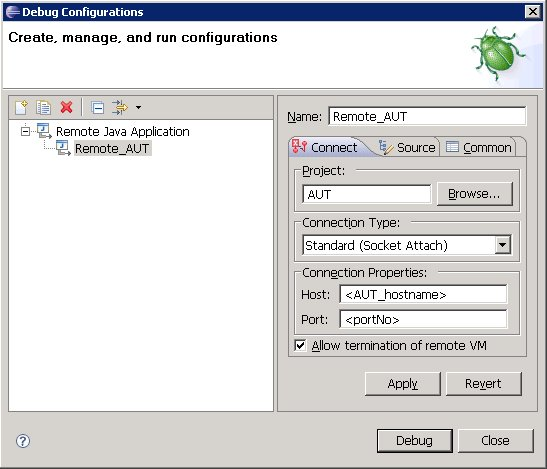
\includegraphics[width=\textwidth]{Debugging/PS/eclipseRemoteDebug}
\caption{Launching eclipse remote debug application}
\label{EclipseRemoteDebugging}
\end{figure}

To get your \gdaut{} running using remote debugging options you have to take the following steps:
\begin{enumerate}
 \item Start the \gdagent{}
 \item Connect the \ite{} with the \gdagent{}, load the \gdproject{} in \app{} and invoke the startup of the \gdaut{} in the \ite{}.
 \item If ''suspend=y'', you now have to run your "Remote Java Application"-configuration 
 in Eclipse, as the JVM is waiting for the debugger to connect before starting the 
 application. As soon as you are connected you should see the default debug behaviour in your
 debug perspective of Eclipse.
 \item Your \gdaut{} has now been launched with the ability to use remote debugging.  
\end{enumerate}

If you wish to debug an RCP \gdaut{}  which is launched with an 
executable file, you must pass these JRE arguments via the \gdaut{} arguments and ''-vmargs''. When using this option, make sure you overwrite all JRE options that are defined in the ''config.ini'' of your RCP launcher.
